\section{Pumps }\label{pumps}

The water pump is quite simply the component that drives the flow in plant and condenser loops. How it reacts depends on several different conditions. In total, there are three different decision variables, two of which are defined by user input. These three deciding factors are whether the pump is constant or variable speed, whether the pump operation is continuous or intermittent, and whether or not there is a load on the loop. The pump is simulated first on the supply side loop after the demand side loop has determined what the demand on the loop will be. For further reference look at sections Pump Control for Plant and Condenser Loops, Plant/Condenser Supply Side, and Plant/Condenser Demand Side in the Plant Flow Resolver of this document.

\subsection{Summary of Pump Rules}\label{summary-of-pump-rules}

\begin{itemize}
\item
  Pumps in Plant Loop can be on the supply side or demand side
\item
  A Pump, if present, in the demand side of plant loop must be the first component of the inlet branch.
\item
  Pumps in Condenser loop must be on supply side
\item
  Pumps can operate as constant or variable flow.
\item
  Pumps can run continuously or intermittently.
\item
  Single boiler/chiller with NO bypass, use Pump:ConstantSpeed
  \begin{itemize}
\item
  Boiler/chiller should be constant flow
\item
  Pump should be intermittent
  \end{itemize}
\item
  Single boiler/chiller with NO bypass, Pump:VariableSpeed
  \begin{itemize}
\item
  Boiler/chiller should be variable flow, regardless of whether pump is intermittent or continuous (runs at the minimum if demand is less than minimum, this includes zero.)
  \end{itemize}
\item
  Single boiler/chiller with bypass, Pump:ConstantSpeed
  \begin{itemize}
\item
  Boiler/chiller can be constant or variable flow
\item
  Pump may be intermittent or continuous as long as the bypass can handle the entire pump volume when the boiler is not operating
  \end{itemize}
\end{itemize}

Multiple branches add more complexity, but it is nothing more than continuity. If the pump is putting out flow then it has to have a branch to flow down whether it is a chiller or a bypass. It can be safer to add the bypass for a simulation. If the active machines require the flow the bypass will be dry. If performing a pressure simulation, and the flow goes through a machine which is off, the pressure drop will be accounted for, but no heat transfer through the machine will be calculated.

If the user designates a pump that is operating continuously, the pump will run regardless of whether or not there is a load. This may have the net effect of adding heat to the loop if no equipment is turned on. If the pump operates intermittently, the pump will run at its capacity if a load is sensed and will shut off if there is no load on the loop. If the pump is scheduled, the schedule modifies the Rated Volumetric Flow Rate of the pump on a time basis. The default is that the pump is ON and runs according to its other operational requirements.

Shown below is pseudo code for the calculation of the total efficiency of the pump and the actual pumping efficiency when the motor efficiency is accounted for either variable or constant volume pumps.

~~~~!~ Total~Efficiency \% = Rated~Volume~Flow~Rate * Rated~Pump~Head / Rated~Power~Use

~~~~TotalEffic = PumpEquip(PumpNum)\%NomVolFlowRate *~~~\&

~~~~~~~~~~~~~~~~~~~~~ PumpEquip(PumpNum)\%NomPumpHead /~\&

~~~~~~~~~~~~~~~~~~~~~ PumpEquip(PumpNum)\%NomPowerUse

~~~~!~ Calculated~Pump~Efficiency \% = Total~Efficiency \% / Motor~Efficiency \%

~~~~PumpEquip(PumpNum)\%PumpEffic = TotalEffic /

~~~~~~~~~~~~~~~~~~~~~~~~~~~~~~~~~~~ PumpEquip(PumpNum)\%MotorEffic

\subsection{Dynamic Pump Pressure Head}\label{dynamic-pump-pressure-head}

There is an option when performing plant/condenser loop simulations to account for dynamically changing loop pressure drop. For the current implementation, the loop pressure drop is calculated based on pressure drop data on each branch of the loop, then this total pressure drop is set as the pump pressure head. There is no pump curve implemented yet, so it is assumed that the pump can always handle this pressure value. This is a first approximation to actually having the pump ride a curve, and this initial implementation allows the user to enter minimal data, and yet get a more dynamic output for pump power, which is calculated based on current pressure drop and flow rate. The equation for pump power is now:

\begin{equation}
Pump~Electric~Power = Pump~Volume~Flow~Rate*\frac{{Pump~Head}}{{Total~Efficiency}}
\end{equation}

Without the pressure simulation, the pump power is based on the rated value entered with the pump object. For further information, see the input-output reference for Branch objects, and PlantLoop/CondenserLoop objects; as well as the Plant/Condenser loop section of this engineering reference.

\subsection{Variable Speed Pump}\label{variable-speed-pump}

A variable speed pump (object name: Pump:VariableSpeed) is defined with maximum and minimum flow rates that are the physical limits of the device. The pump will operate and select a flow somewhere between the minimum and maximum limits. In the case where the pump is running, the pump will try to meet the flow request made by demand side components.

All of the pump rules and efficiency and power calculations are applicable from the introduction in the pump group section. The main difference between the the variable volume pump and the constant volume pump is the Part Load Performance Curve.The fraction of full load power is determined by the cubic equation:

\begin{equation}
FractionFullLoadPower = {C_1} + {C_2}PLR + {C_3}PL{R^2} + {C_4}PL{R^3}
\end{equation}

where C\(_{1}\),C\(_{2}\),C\(_{3}\),and C\(_{4}\) are Coefficients 1 -- 4 and PLR is the Part Load Ratio. In the pseudo code below, the FracFullLoadPower modifies the NomPowerUse for the total pump ``Power'' and shows the ``ShaftPower'' and the ``PumpHeattoFluid''.

~~~~VolFlowRate = PumpMassFlowRate / LoopDensity

~~~~PartLoadRatio = VolFlowRate / PumpEquip(PumpNum)\%NomVolFlowRate

~~~~FracFullLoadPower = PumpEquip(PumpNum)\%PartLoadCoef(1)~~~~~~~~~~~~~~~~~~~~ \&

~~~~~~~~~~~~~~~~~~~~~ + PumpEquip(PumpNum)\%PartLoadCoef(2) * PartLoadRatio~~~~ \&

~~~~~~~~~~~~~~~~~~~~~ + PumpEquip(PumpNum)\%PartLoadCoef(3) * PartLoadRatio**2 \&

~~~~~~~~~~~~~~~~~~~~~ + PumpEquip(PumpNum)\%PartLoadCoef(4) * PartLoadRatio**3

~~~~Power = FracFullLoadPower * PumpEquip(PumpNum)\%NomPowerUse

~~~~ShaftPower = Power * PumpEquip(PumpNum)\%MotorEffic

~~~~! This adds the pump heat based on User input for the pump

~~~~! We assume that all of the heat ends up in the fluid eventually since this is a closed loop

~~~~!~ PumpHeattoFluid = ShaftPower*(1-PumpEquip(PumpNum)\%PumpEffic)

~~~~PumpHeattoFluid = ShaftPower + (Power - ShaftPower) \& \par
\hspace{5cm} *PumpEquip(PumpNum)\%FracMotorLossToFluid

~~~~Node(OutletNode)\%Temp = Node(InletNode)\%Temp \& \par
\hspace{6cm} + PumpHeattoFluid/(PumpMassFlowRate * LoopCp)

~~~~PumpEquip(PumpNum)\%Power = Power

\subsection{Pressure-based Flow for Variable Speed Pumps}\label{pressure-based-flow-for-variable-speed-pumps}

With the introduction of pressure simulations in plant loops, the variable speed pump object now has the capability to model a more realistic variable speed operation. There are two operation modes which are introduced: differential pressure control is a widely used VFD control method while most VFDs also have a manual control mode in which the user determines the input frequency of the electric motor. The mode can be selected as `ManualControl' or `PressureSetpointControl' in the VFD Control Type input in Pump:VariableSpeed objects.

In manual VFD control mode the specified schedule will determine the current pump rotational speed throughout the simulation. This RPM value will be used to scale the pump curve which is entered by the user in non-dimensional form. Once the pump curve has been fixed then the successive substitution method will use this curve with the system curve to resolve the operating point. VFD manual control mode is implemented in EnergyPlus with the use of the RPM schedule input.

Differential pressure based control will maintain the differential pressure within the specified range. The pressure drop corresponding to the mass flow request will be calculated using the effective pressure constant of the system. This pressure drop will be checked against the pressure set point range. If the pressure drop is within the user specified range, then the mass flow rate will be checked against mass flow rates of operating points corresponding to maximum and minimum rotational speeds. Maximum and minimum differential pressure and rotational speeds are schedule inputs and can be entered as constant schedule.

The allowable mass flow rate range for the Differential pressure control is explained in the Figure~\ref{fig:allowable-mass-flow-rate-range-for}.

\begin{figure}[hbtp] % fig 265
\centering
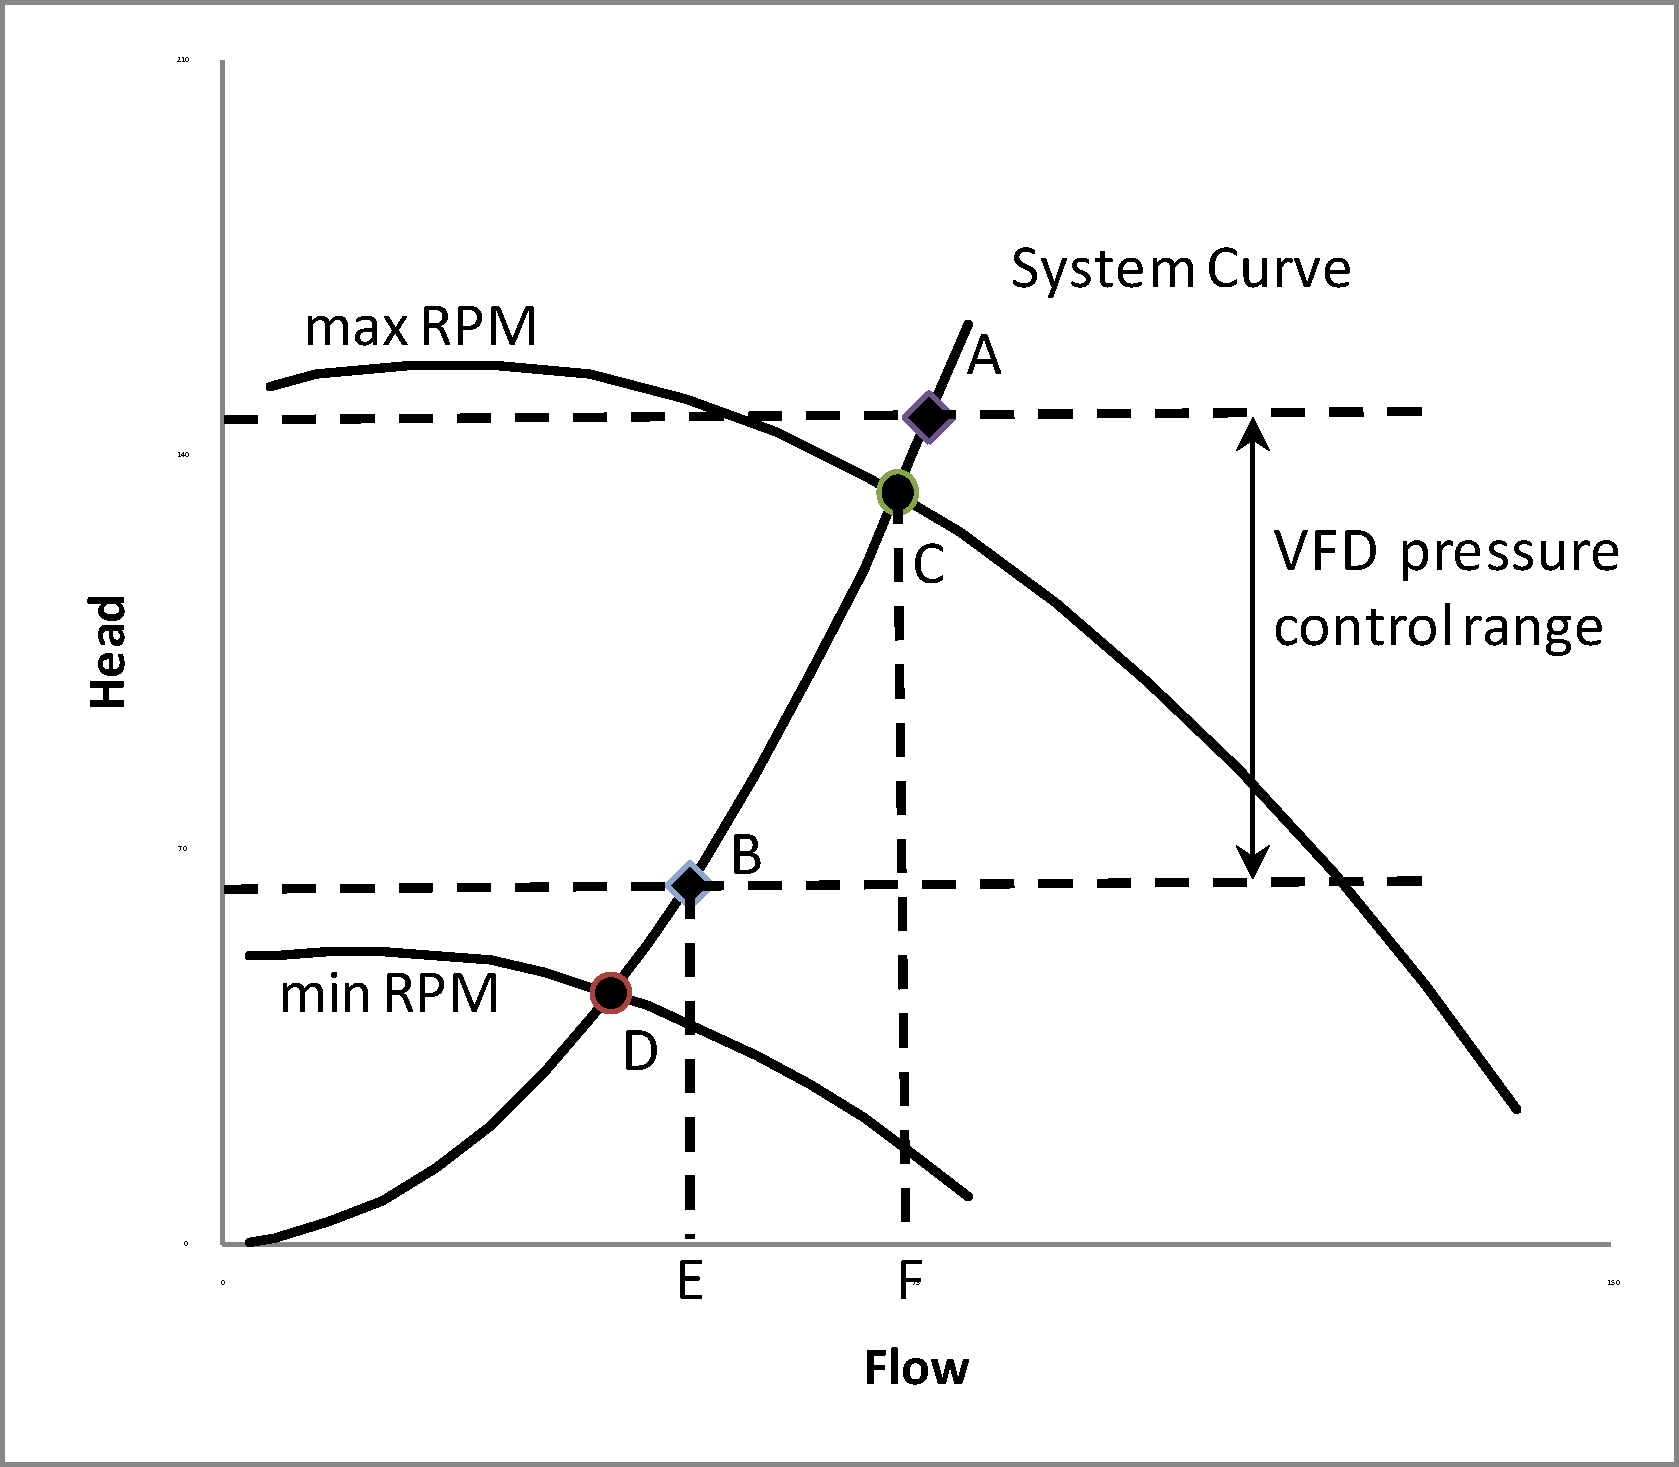
\includegraphics[width=0.9\textwidth, height=0.9\textheight, keepaspectratio=true]{media/image5856.png}
\caption{Allowable mass flow rate range for the Differential pressure control \protect \label{fig:allowable-mass-flow-rate-range-for}}
\end{figure}

\subsection{Constant Speed Pump}\label{constant-speed-pump}

The operation of a constant speed pump (object name: Pump:ConstantSpeed) is fairly straightforward. The user designates a maximum flow rate and when this pump operates it will run at that capacity. The main difference between the constant speed pump and the variable speed pump is that the fraction of full load power is always = 1. In the pseudo code below, the FracFullLoadPower is = 1.0, therefore the Power is always the full power.

~~~~VolFlowRate = PumpMassFlowRate / LoopDensity

~~~~PartLoadRatio = VolFlowRate / PumpEquip(PumpNum)\%NomVolFlowRate

~~~~FracFullLoadPower = 1.0

~~~~Power = FracFullLoadPower * PumpEquip(PumpNum)\%NomPowerUse

~~~~ShaftPower = Power * PumpEquip(PumpNum)\%MotorEffic

~~~~! This adds the pump heat based on User input for the pump

~~~~! We assume that all of the heat ends up in the fluid eventually since this is a closed loop

~~~~! PumpHeattoFluid = ShaftPower*(1-PumpEquip(PumpNum)\%PumpEffic)~ \&

~~~~PumpHeattoFluid = ShaftPower + (Power - ShaftPower)~\& \par
\hspace{5cm} * PumpEquip(PumpNum)\%FracMotorLossToFluid

~~~~Node(OutletNode)\%Temp = Node(InletNode)\%Temp \& \par
\hspace{6cm} + PumpHeattoFluid/(PumpMassFlowRate * LoopCp)

~~~~PumpEquip(PumpNum)\%Power = Power

\subsection{Pressure-based Flow for Constant Speed Pumps}\label{pressure-based-flow-for-constant-speed-pumps}

The constant speed pump can flow can also be overridden dynamically based on a response to the plant loop pressure drop. In ``single-loop-pump'' simulations (no branch pumps, no common pipe), the user can enter a dimensionless pump curve on the Pump:ConstantSpeed (see I/O ref) object which represents the single speed pressure-flow relationship of the pump. In the process of determining the operating flow rate for the pump, the pump will check to see if a valid pressure simulation is being performed. If it is, a flow will be prescribed based on a resolution between system pressure characteristics and the pump pressure curve. This will cause the pump flow to be ``unpredictable,'' meaning that it will not always be a constant, expected value, which is basically what the constant speed pump gives you without the pressure simulation. There is more detail on the pressure based simulation in the Plant/Condenser loop sections of this documentation.

\subsection{Pump Heat Addition to the Loop}\label{pump-heat-addition-to-the-loop}

Due to the fact that a pump is a mechanical device that acts on the fluid it is circulating, it causes the fluid to increase in temperature. The EnergyPlus model assumes that all pressure increase caused by the pump will eventually be lost due to friction, and that friction will be added as heat to the fluid. Since the plant and condenser loops are not yet true pressure-based models, EnergyPlus assumes that all of the heat resulting from the pump itself and from friction throughout the loop. Therefore, as of version 7, the pump heat is added to the plant loop interface by injecting the heat into the mixed tanks used to model loop thermal capacitance(previously it was added at the outlet node of the pump). The amount of heat added to the fluid is calculated using the following two equations:

\begin{equation}
ShaftPower = PumpPower * PumpMotorEfficiency
\end{equation}

\begin{equation}
PumpHeatToFluid = ShaftPower + \left( {PumpPower - ShaftPower} \right) * FracMotorLossToFluid
\end{equation}

where the pump motor efficiency is defined by the user input and the FracMotorLossToFluid is the amount of heat generated by the pump motor that is added to the fluid loop (as opposed to being lost to the environment where the pump is located). FracMotorLossToFluid is also a user input.

Note that the shaft power relates to the increase in head through the pump. Since all of this head is lost through the piping network due to frictional heat, this represents a heat gain by the fluid throughout the network. For simplicity, this heat is added along with the heat resulting from the pump motor. The difference between the pump power and the shaft power is the inefficiency of the pump---or the amount of energy input into the pump that the motor converts to heat rather than mechanical energy. Some of this heat is added to the fluid being pumped. These two terms are shown in the PumpHeatToFluid equation shown above. Since EnergyPlus Version 7, this heat is added to the loop capacitance tank(s) rather than at the pump's outlet and so the outlet temperature is equal to the inlet temperature.

\subsection{Pump Heat Addition to Surrounding Zone}\label{pump-heat-addition-to-surrounding-zone}

If the user input includes naming a Zone that surrounds the pump, then the pump becomes a source of internal heat gain to that zone.~ The amount of heat transmitted to the surrounding zone is simply the difference between power input and the rate of heat transferred to the fluid. The user can also input a fraction, \({f_{rad}}\), that controls the overall split between thermal radiation and sensible convection.~ The pump's sensible zone gains are determined using the following equations:

\begin{equation}
TotalZoneGain = PumpPower - PumpHeatToFluid
\end{equation}

\begin{equation}
ConvectiveZoneGain = \left( {1 - {f_{rad}}} \right)*TotalZoneGain
\end{equation}

\begin{equation}
RadiativeZoneGain = {f_{rad}}*TotalZoneGain
\end{equation}

\subsection{Headered Pumps}\label{headered-pumps}

The input objects HeaderedPumps:ConstantSpeed and HeaderedPumps:VariableSpeed ~provide models for headered pumps that consist of two or more pumps connected in parallel. The headered pump is simulated as a single component, and it is specified as an integer number of a specific pump. The flow rate provided by the headered pump is determined by the number of pumps in operation and the flow rate of the individual pump. The total flow rate is calculated as

\begin{equation}
FlowProvided = NumPumpsON*IndividualPumpFlowRate
\end{equation}

The simulation starts by turning ON all pumps in the group. The pumps are then turned OFF one at a time until the flow provided is less than the flow requested. Finally the last pump is turned back ON to meet the remaining flow (FlowDifference) requested. The flow rate of the last pump depends on the pump bank type. For constant speed headered pumps, the last pump runs at the nominal flow rate, thereby giving a final headered pump flow which is equal to or greater than the flow requested. In a variable speed headered pump the last pump runs at part load so that the flow provided matches the flow requested. The power of the headered pump is then calculated as

\begin{equation}
Power = (P{R_{FL}}{\rm{*N}}{}_{{\rm{FL}}} + {\rm{P}}{{\rm{R}}_{{\rm{PL}}}}{\rm{*}}{{\rm{N}}_{{\rm{PL}}}}{\rm{)*}}{{\rm{P}}_{{\rm{Nom}}}}{\rm{  }}
\end{equation}

where:

\emph{Power} is the power consumed by the pump bank

\emph{PR\(_{FL}\)} is the power ratio at full load (generally equal to 1)

\emph{N\(_{FL}\)} is the number of pumps running at full load

\emph{PR\(_{PL}\)} is the power ratio at part load

\emph{N\(_{PL}\)} is the number of pumps running at part load

\emph{P\(_{Nom}\)} is the nominal power consumption of individual pumps.

For a constant speed headered pump, \emph{N\(_{PL}\)} is zero. For a variable speed headered pump, \emph{N\(_{PL}\)} is equal to one.

\subsection{Condensate Pumps}\label{condensate-pumps}

The input object Pump:VariableSpeed:Condensate provides a model for steam condensate pumps, see the discussion for steam loops, reference: Condensate Pump.
